\documentclass{article}
\setlength{\parskip}{1em}
\usepackage{amsmath}
\usepackage{listings}
\usepackage{graphicx}
\graphicspath{ {./images/} }
\allowdisplaybreaks

\begin{document}

\centerline{\sc \large Reaction Wheel Stabilized Inverted Pendulum}
\vspace{.25pc}
\centerline{\sc \small optimal control, state space, and quaternions, oh my}
\vspace{.5pc}
\centerline{\sc Trent Fehl}
\vspace{1pc}

\begin{abstract}
In an attempt to develop some new skills, I started development of an 
inverted pendulum. This paper describes the system and the optimal 
controller development for the reaction wheel stabilized inverted pendulum.
Not included in this paper is the printed circuit board design, part 
selection, CAD models for the wheels, and machine paths for wheel manufacture.
I drew from papers concerning optimal control of a cart stabilized inverted 
pendulum, PID control of a reaction wheel stabilized inverted pendulum, 
and finally satellite control systems papers that utilize quaternions.
\end{abstract}

\section*{System Description}
\noindent This inverted pendulum is stabilized by the spinning of reaction wheels
mounted to the end of the pendulum. Only the case of a pendulum which is 
initiated and is controlled to its inverted position is being considered.
In addition to the wheels at the end of the pendulum rod, there is mass
associated with motors, a printed circuit board, batteries, and structure.
Theses are not shown in the image below but their masses are configurable 
variables for the control system.

\begin{figure}[h]
\centering
\begin{minipage}{.5\textwidth}
 \centering
 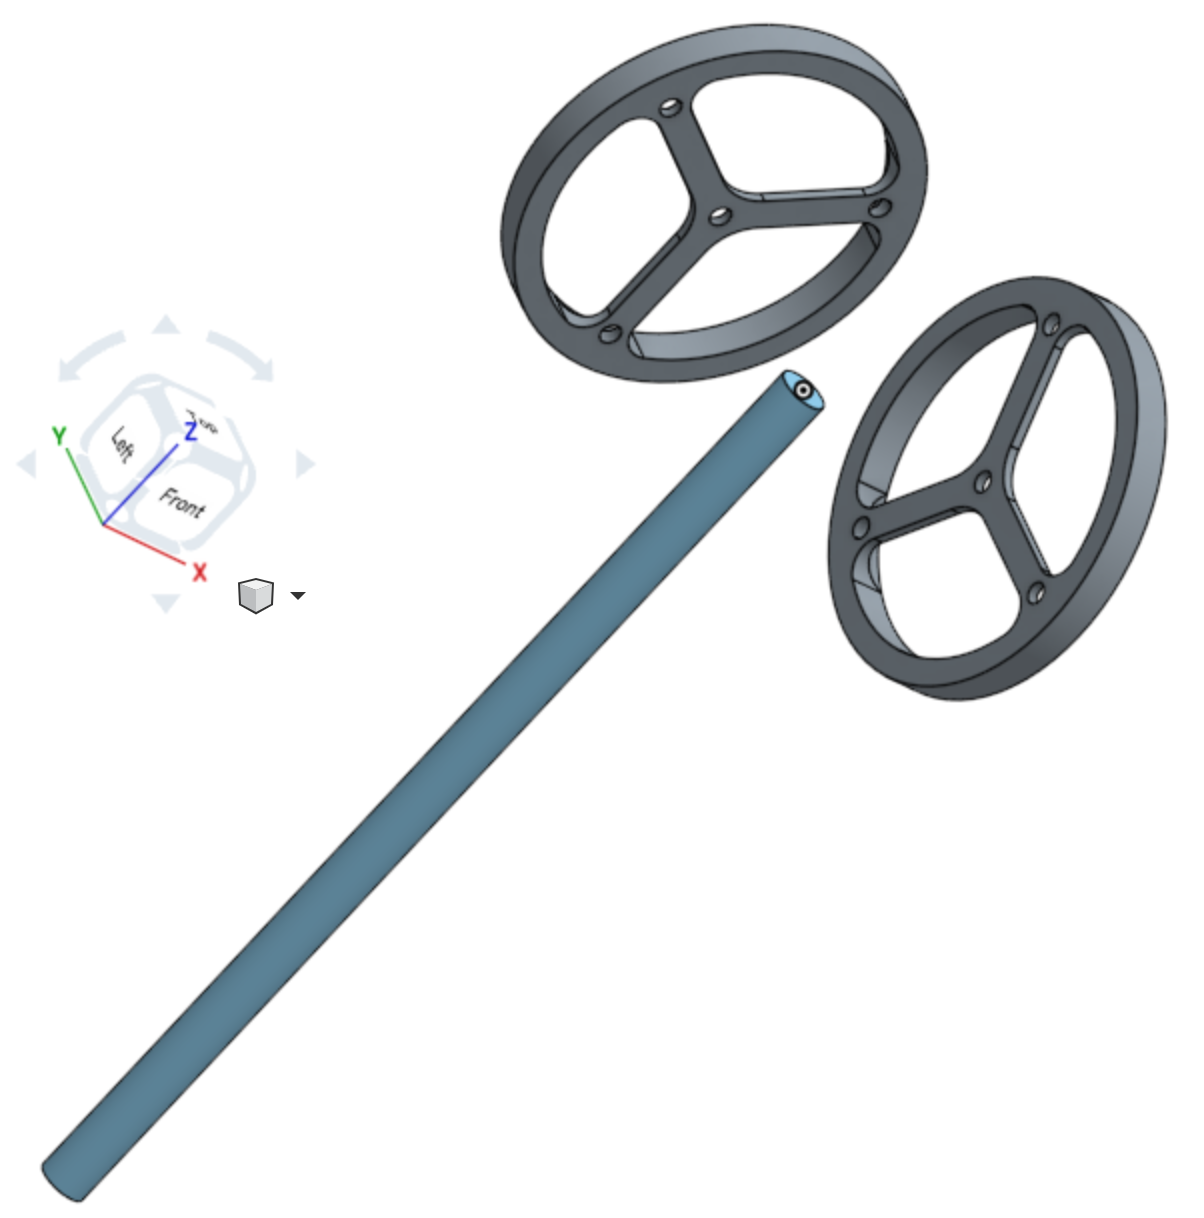
\includegraphics[width=1\linewidth]{system_angle}
 \caption{System rotated.}
\end{minipage}%
\begin{minipage}{.5\textwidth}
 \centering
 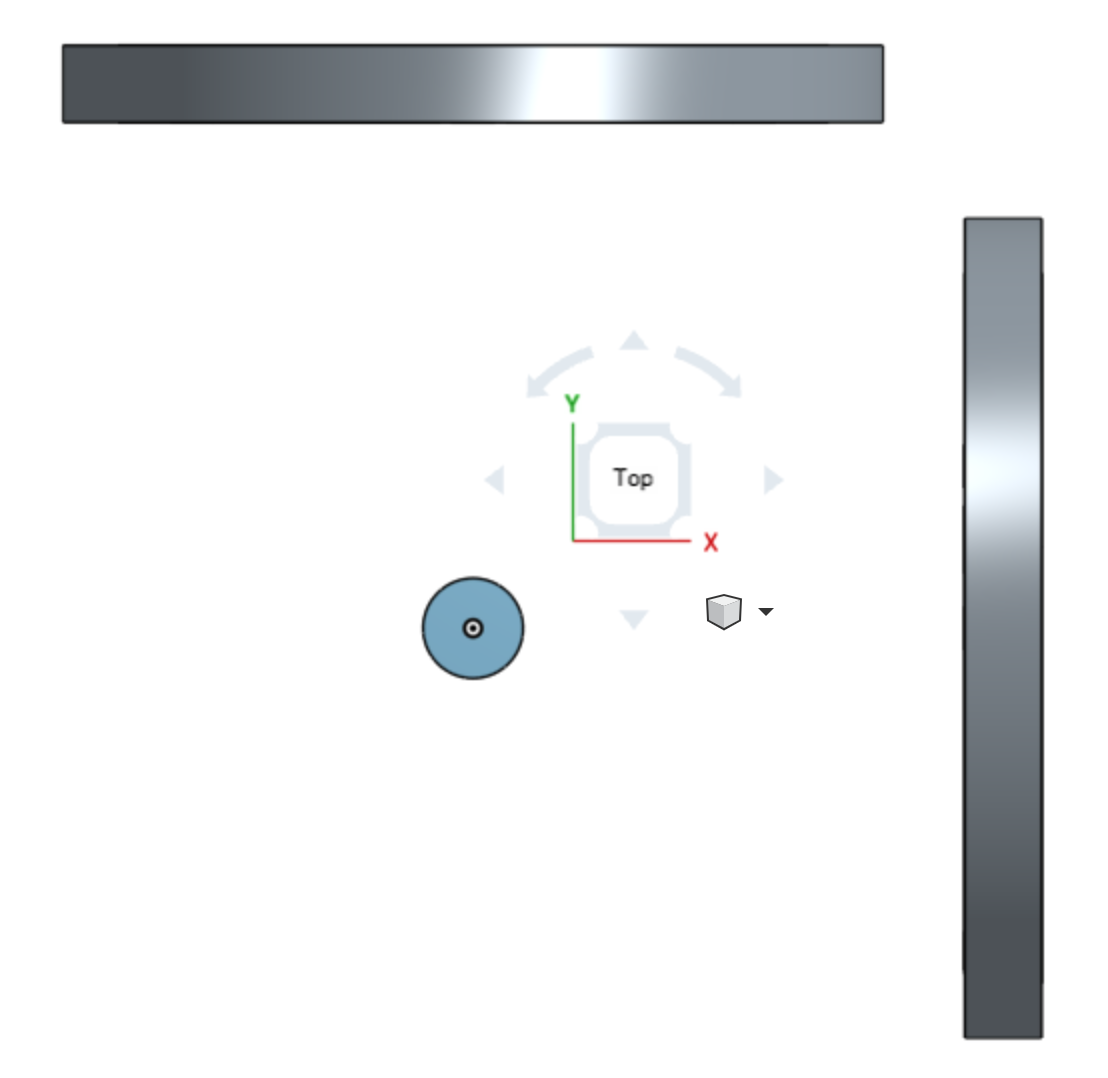
\includegraphics[width=1\linewidth]{system_top}
 \caption{Top of system.}
\end{minipage}
\end{figure}

\noindent The equations of motion were determined and are described below.
These equations are used to build a state space representation
of the system. The state space representation takes the form 
$\boldsymbol{\dot{x}(t)} = \boldsymbol{A}\boldsymbol{x(t)} + 
\boldsymbol{B}\boldsymbol{u(t)}$ where $x(t)$ is the system state 
at time $t$, $u(t)$ is the input to the system at time $t$, and $A$ 
and $B$ are their respective coefficients. Below are the expanded 
matrices with our variables $\omega$, rotational speed for the 
respective axis and quaternions represented by $\boldsymbol{q} = q_0 + q_1\,i 
+ q_2\,j + q_3\,k$. $\boldsymbol{q}$ and $\boldsymbol{w}$ are measured 
by a 3-axis accelerometer and a 3-axis gyroscope, respectively.

\[
\begin{bmatrix}
\underset{3\times 1}{\boldsymbol{\dot{q}}} \\
\underset{3\times 1}{\boldsymbol{\dot{\omega}_p}} \\
\underset{3\times 1}{\boldsymbol{\dot{\omega}_w}}
\end{bmatrix}
=
\begin{bmatrix}
\underset{3\times 3}{\boldsymbol{0}} & \underset{3\times 3}{\boldsymbol{A_{12}}} & \underset{3\times 3}{\boldsymbol{0}} \\
\underset{3\times 3}{\boldsymbol{A_{21}}} & \underset{3\times 3}{\boldsymbol{A_{22}}} & \underset{3\times 3}{\boldsymbol{A_{23}}} \\
\underset{3\times 3}{\boldsymbol{0}} & \underset{3\times 3}{\boldsymbol{0}} & \underset{3\times 3}{\boldsymbol{A_{33}}}
\end{bmatrix}
\begin{bmatrix}
\underset{3\times 1}{\boldsymbol{q}} \\
\underset{3\times 1}{\boldsymbol{\omega_p}} \\
\underset{3\times 1}{\boldsymbol{\omega_w}}
\end{bmatrix}
+
\begin{bmatrix}
\underset{3\times 3}{\boldsymbol{0}} \\
\underset{3\times 3}{\boldsymbol{B_{21}}} \\
\underset{3\times 3}{\boldsymbol{B_{31}}}
\end{bmatrix}
\begin{bmatrix}
\underset{3\times 1}{\boldsymbol{\mu}}
\end{bmatrix}
\]

\noindent See \cite{mitstatespace} for more information about this representation.

\section*{\small Quaternion Equations}
\[
\begin{bmatrix}
\dot{q}_0 \\
\dot{q}_1 \\
\dot{q}_2 \\
\dot{q}_3
\end{bmatrix}
=
\frac{1}{2}
\begin{bmatrix}
q_0 & -q_1 & -q_2 & -q_3 \\
q_1 & q_0 & -q_3 & q_2 \\
q_2 & q_3 & q_0 & -q_1 \\
q_3 & -q_2 & q_1 & q_0 \\
\end{bmatrix}
\begin{bmatrix}
0 \\
\omega_1 \\
\omega_2 \\
\omega_3
\end{bmatrix}
\]

\noindent The above is apparently from \cite{noaccess} but I was not able to
get access to it. It makes sense though: The rate of change in
attitude should have the same units as angular speed times an
attitude. In the equation below we simply zero-out the $\dot{q}_0$
term and substitute in for $q_0$ using $q_0 = \sqrt{1 - q_1^2 
- q_2^2 - q_3^2}$. This reduces the number of terms in the equation
and per \cite{quatsforspacecraft} is still controllable.

\[
\begin{bmatrix}
\dot{q}_1 \\
\dot{q}_2 \\
\dot{q}_3
\end{bmatrix}
=
\frac{1}{2}
\begin{bmatrix}
\sqrt{1 - q_1^2 - q_2^2 - q_3^2} & -q_3 & q_2 \\
q_3 & \sqrt{1 - q_1^2 - q_2^2 - q_3^2} & -q_1 \\
-q_2 & q_1 & \sqrt{1 - q_1^2 - q_2^2 - q_3^2}
\end{bmatrix}
\begin{bmatrix}
\omega_1 \\
\omega_2 \\
\omega_3
\end{bmatrix}
\]

\noindent Finally we linearlize this using small angle approximation and the 
Taylor series expansion with the following equation. 

$$\boldsymbol{q} = \left[ q_0, q_1, q_2, q_3 \right]^T 
= \left[ \cos\frac{\theta}{2}, \boldsymbol{\hat{e}}^T\sin\frac{\theta}{2} \right]^T$$ 

\noindent We can do this if we assume the pendulum system is started in appoximately 
the upright position and maintains that attitude. The Taylor series expansion 
is then centered around $\theta = 0$, reducing the $\sin\frac{\theta}{2}$ terms to $0$.

\[
\begin{bmatrix}
\dot{q}_1 \\
\dot{q}_2 \\
\dot{q}_3
\end{bmatrix}
=
\frac{1}{2}
\begin{bmatrix}
1 & 0 & 0\\
0 & 1 & 0 \\
0 & 0 & 1
\end{bmatrix}
\begin{bmatrix}
\omega_1 \\
\omega_2 \\
\omega_3
\end{bmatrix}
\]

\section*{\small Angular Rotation Equations}
\noindent Again using the small angle approximation we can write the equation
of motion for the change in rotational speed in terms of quaterions.

$$\dot{\omega}_{px}\; =\;
\frac{-b_{wx}}{I_{px}}\,\omega_{wx}\;
+ \frac{b_{px}}{I_{px}}\,\omega_{px}\;
+ \frac{2glm}{I_{px}}\,q_1\;
+ \frac{k_s}{I_{px}}\,\mu$$

$$\dot{\omega}_{py}\; =\;
\frac{-b_{wy}}{I_{py}}\,\omega_{wy}\;
+ \frac{b_{py}}{I_{py}}\,\omega_{py}\;
+ \frac{2glm}{I_{py}}\,q_2\;
+ \frac{k_s}{I_{py}}\,\mu$$

\noindent The third equation does not have to be solved for basic operation because
we're not controlling around that axis. Below is what I think may work if 
a third wheel was added. $F_{spin}$ is a term that covers force of rotation around
the Z-axis while the pendulum is not vertical. We can simply set it equal
to 1 for this simulation.

$$\dot{\omega}_{pz}\; =\;
\frac{-b_{wy}}{I_{pz}}\,\omega_{wz}\;
+ \frac{b_{pz}}{I_{pz}}\,\omega_{pz}\;
+ \frac{2gF_{spin}}{I_{pz}}\,q_3\;
+ \frac{k_s}{I_{pz}}\,\mu$$

\noindent Working our way through the terms on the right side of the equal 
sign we have force from friction in the wheel bearings, force from friction
at the pendulum point of rotation, force of gravity pulling the pendulum 
down, and then finally the force of the wheels transferring momentum. The 
terms used are defined here:
\begin{itemize}
\setlength{\itemindent}{.5in}
\item $-b_w$ is the friction in the wheel bearings.
\item $\omega_w$ is rotational speed of the wheel.
\item $I_p$ is the moment of inertia of the pendulum system.
\item $b_p$ is the friction in the rotation of the pendulum rod.
\item $\omega_p$ is the rotational speed of the pendulum rod.
\item $g$ is gravitational acceleration (-9.81 $m/s^2$).
\item $l$ is the length of the pendulum rod.
\item $m$ is the combined mass at the end of the pendulum rod.
\item $k_s$ is the voltage applied to the motor.
\end{itemize}

\noindent Finally we have the equation for the rate of change of the 
reaction wheel rotational speed. There are two terms to account for 
here: friction in the wheel bearings and torque into the wheels from
the motor that we are controlling.

$$\dot{\omega}_{wx}\; =\;
\frac{-b_{wx}}{I_{wx}}\,\omega_{wx}\;
+ \frac{k_s}{I_{wx}}\,\mu$$

$$\dot{\omega}_{wy}\; =\;
\frac{-b_{wy}}{I_{wy}}\,\omega_{wy}\;
+ \frac{k_s}{I_{wy}}\,\mu$$


\noindent Where $I_w$ is the moment of inertia of the wheel.

\section*{\small Final State and Input Matrices}
Taking the equations from the previous two sections we can build
out the original state matrices.

$$\boldsymbol{A_{12}} = \frac{1}{2}\boldsymbol{I_3}$$

\begin{align*}
\boldsymbol{A_{21}} &=
\begin{bmatrix}
\frac{2glm}{I_{px}} & 0 & 0 \\[1em]
0 & \frac{2glm}{I_{py}} & 0 \\[1em]
0 & 0 & \frac{2gF_{spin}}{I_{pz}}
\end{bmatrix}
&
\boldsymbol{A_{22}} &=
\begin{bmatrix}
\frac{B_{px}}{I_{px}} & 0 & 0 \\[1em]
0 & \frac{B_{py}}{I_{py}} & 0 \\[1em]
0 & 0 & \frac{B_{pz}}{I_{pz}}
\end{bmatrix}\\[2em]
\boldsymbol{A_{23}} &=
\begin{bmatrix}
-\frac{B_{wx}}{I_{px}} & 0 & 0 \\[1em]
0 & -\frac{B_{wy}}{I_{py}} & 0 \\[1em]
0 & 0 & -\frac{B_{wz}}{I_{pz}}
\end{bmatrix}
&
\boldsymbol{A_{33}} &=
\begin{bmatrix}
-\frac{B_{wx}}{I_{wx}} & 0 & 0 \\[1em]
0 & -\frac{B_{wy}}{I_{wy}} & 0 \\[1em]
0 & 0 & -\frac{B_{wz}}{I_{wz}}
\end{bmatrix}\\[2em]
\boldsymbol{B_{21}} &=
\begin{bmatrix}
\frac{k_s}{I_{px}} & 0 & 0 \\[1em]
0 & \frac{k_s}{I_{py}} & 0 \\[1em]
0 & 0 & \frac{k_s}{I_{pz}}
\end{bmatrix}
&
\boldsymbol{B_{31}} &=
\begin{bmatrix}
\frac{k_s}{I_{wx}} & 0 & 0 \\[1em]
0 & \frac{k_s}{I_{wy}} & 0 \\[1em]
0 & 0 & \frac{k_s}{I_{wz}}
\end{bmatrix}\\
\end{align*}

\section*{Controller Development}
Here the controller design work will be described.

\section*{Software Operation}
The simulation software was developed on Mac OSX and Python 3.5.

\section*{\small Setup and Execution}
\noindent The user of this script should first set up a profile 
in the config files that represents the motors, pendulum, and 
wheels that they wish to simulate. They then need to update the 
three lines in pendulum.py where the config is chosen.

\begin{lstlisting}[language=python]
# Set configuration
motor = config_motor.maxon_70w
wheel = config_wheel.estimate
pend = config_pendulum.estimate
\end{lstlisting}

\noindent The script can then be invoked with:
\begin{lstlisting}[language=bash]
$ python pendulum.py
\end{lstlisting}

\section*{\small Output}
\noindent The output will provide the user with the K values and 
a plot of the simulated control given the initial gains and starting
position of the pendulum. Below is the output from a simulation using
the default initialization.

\begin{figure}
\centering
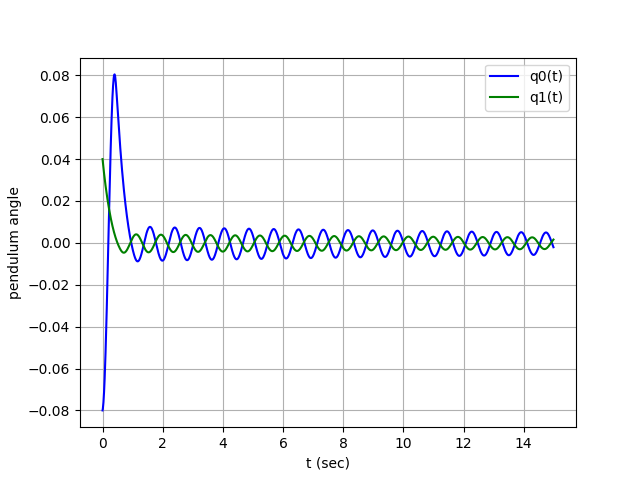
\includegraphics[width=1\linewidth]{time_series_default}
\end{figure}

\begin{figure}
\centering
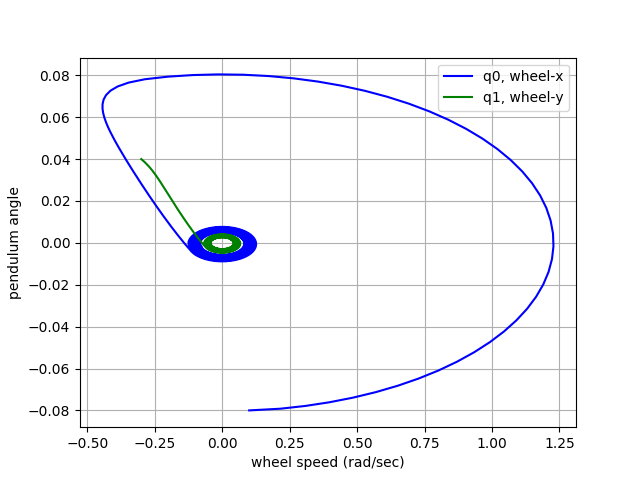
\includegraphics[width=1\linewidth]{parametric_default}
\end{figure}

\begin{thebibliography}{9}
\bibitem{mitstatespace} 
State-Space Representation of LTI Systems, Derek Rowell October 2002
\\\texttt{http://web.mit.edu/2.14/www/Handouts/StateSpace.pdf}

\bibitem{quatsforspacecraft} 
Yaguang Yang,
\textit{Quaternion based model for momentum biased nadir pointing spacecraft}, 
Aerospace Science and Technology 14 (2010) 199–202

\bibitem{noaccess} 
B. Wie, 
\textit{Vehicle Dynamics and Control}, 
AIAA Education Series, AIAA, Reston, VA, 1998.
\end{thebibliography}

\end{document}
